\documentclass[11pt,letterpaper]{article}

\usepackage[letterpaper,margin=0.8in,nohead]{geometry}

\usepackage[colorlinks]{hyperref}
\usepackage{url}
\usepackage{breakurl}

\hypersetup{
	colorlinks,
	linkcolor={red},
	citecolor={red},
	urlcolor={blue}
}

\usepackage{verbatim}
\usepackage{fancyvrb}
\usepackage{scrextend}
\usepackage{enumitem}
\usepackage{url}
\usepackage{subcaption}

\usepackage{filecontents}
%\usepackage{natbib}
%\nobibliography*

\usepackage{caption}
\usepackage{graphicx}

\usepackage{changepage}   % for the adjustwidth environment

\newenvironment{answer}{\em \color{blue} \begin{adjustwidth}{1cm}{1cm}}{\end{adjustwidth}}

% math
\usepackage{amsthm,amsmath}
\usepackage{amsfonts}

\newcommand{\mc}[1]{\mathcal{#1}}	% Mechanisms / Algorithms
\newcommand{\rv}[1]{\mathbf{#1}}    % Random variable

\newcommand{\pr}[1]{\mathrm{Pr}\{#1\}} % Probability

\newtheorem{corollary}{\bf Corollary}%[theorem]
\newtheorem{lemma}{\bf Lemma}%[theorem]
\newtheorem{definition}{\bf Definition}%[section]

\newtheorem{observation}{\bf Observation}%[theorem]



% load cleveref last!
\usepackage[capitalise]{cleveref}

\crefname{observation}{Observation}{Observations}


\begin{document}
	
	\title{EN3240: Embedded Systems Engineering \\Assignment 4 --- Real Time Scheduling}
	
	%% This is an individual assignment!!
	%% TODO: put your name and index number here!
	\author{Name: Thalagala B. P. \\ Index No: 180631J}
	
	\maketitle
	
	\begin{center}
		\color{red}\bf This is an individual assignment! \\ Due Date: 18 September 2022 by 11.59 PM
	\end{center}
	
	\section*{Instructions}
	%
	
	Please read the instructions and questions carefully. Write your answers directly in the space provided. Compile the tex document and submit the resulting PDF. This is an individual assignment. You are not allowed to take or give any help in completing this assignment.
	
	When drawing images, you may draw them by hand, take a photo and add that as a Figure in LaTeX. Please avoid this option unless you have excellent handwriting and drawing capability!
	
	%%%%%%%%%%%%%%%%%%%%%%%%%%%%%%%%%
	%%%%%%%%%%%%%%%%%%%%%%%%%%%%%%%%%
	\newpage
	%
	Consider the tasks in the following table for scheduling questions in (a), (b) and (c). In the subsequent figures, the first arrival of tasks are shown using * symbol. Use * to indicate subsequent task arrivals. If a task violates its deadline, only abandon that task at the time it violates the deadline, show the violation using `X' mark, and proceed with the next highest priority one. In other words, the `X' mark should be at the same position of * symbol, if violation happens. If the priority of a currently executing task is the same as the priority of a newly arrived task, continue to execute the current task. If the priorities of two tasks are the same and both are ready to execute, then always choose the one with the smaller execution time. The deadline and period values are relative to the arrival time. For example, if a task arrives in time step 2 with a deadline of 8, its actual deadline is timestep 10. Also, if a task arrives in time step 2 with a period of 8, it arrives next in timestep 10.
	
	\begin{table}[h]
		\centering
		\begin{tabular}{|c|c|c|c|c|}
			\hline
			& \textbf{First Arrival} & \textbf{Deadline} & \textbf{Period} & \textbf{Execution Time} \\ \hline
			\textbf{T1} & 0                      & 4                 & 4               & 1                       \\ \hline
			\textbf{T2} & 1                      & 4                 & 4               & 2                       \\ \hline
			\textbf{T3} & 2                      & 5                & 5              & 3                       \\ \hline
		\end{tabular}
	\end{table}
	
	\section*{Problem 1: Real Time Scheduling (2 Points)}
	
	Test whether the tasks are schedulable on a single processor using Rate-Monotonic (RM) scheduling by applying both necessary and sufficiency tests. Indicate whether the test passes or fails.
	
	%% TODO: add answer here
	\subsection*{Sufficiency Test}
	A set of $n$ tasks is schedulable on a uniprocessor by the Rate Monotonic (RM) Scheduling algorithm, if the processor utilization ($\mu$) obey the following inequality.
	\[	\mu \le n\left(2^{\frac{1}{n}} - 1\right) \]
	
	\[
	\mu  	
	= \sum_{i=1}^{3} \frac{c_i}{p_i}
	= \frac{1}{4} + \frac{2}{4} + \frac{3}{5}
	= 1.35
	\]
	
	\[
	n\left(2^{\frac{1}{n}} - 1\right)
	 = 3 \times \left(2^{\frac{1}{3}} - 1\right)
	 = 0.78
	\]
	
According to the obtained values, the sufficient condition for RMS algorithm does not hold for the given tasks. Therefore, the Sufficiency Test fails. This alone does not implies the tasks can not be schedulable. We need to check for the necessary test as well.

\subsection*{Necessary Test}
For uniprocessor, the necessary condition for schedulability,
\[\mu \le 1\]

However, according to the obtained values for $\mu = 1.35$ this necessary test also fails. Therefore it can be concluded that the given three periodic tasks can not be scheduled on  a uni processor using the RMS algorithms.
	%%%%%%%%%%%%%%%%%%%%%%%%%%%%%%%%%
	%%%%%%%%%%%%%%%%%%%%%%%%%%%%%%%%%    
	\newpage
	\section*{Problem 2: Rate Monotonic Scheduling (4 Points)}
	
	Schedule the tasks up to 15 time steps with Rate Monotonic (RM) scheduling.
	
	%% TODO: add answer here
	\begin{figure}[h]
		\centering
		\fbox{
		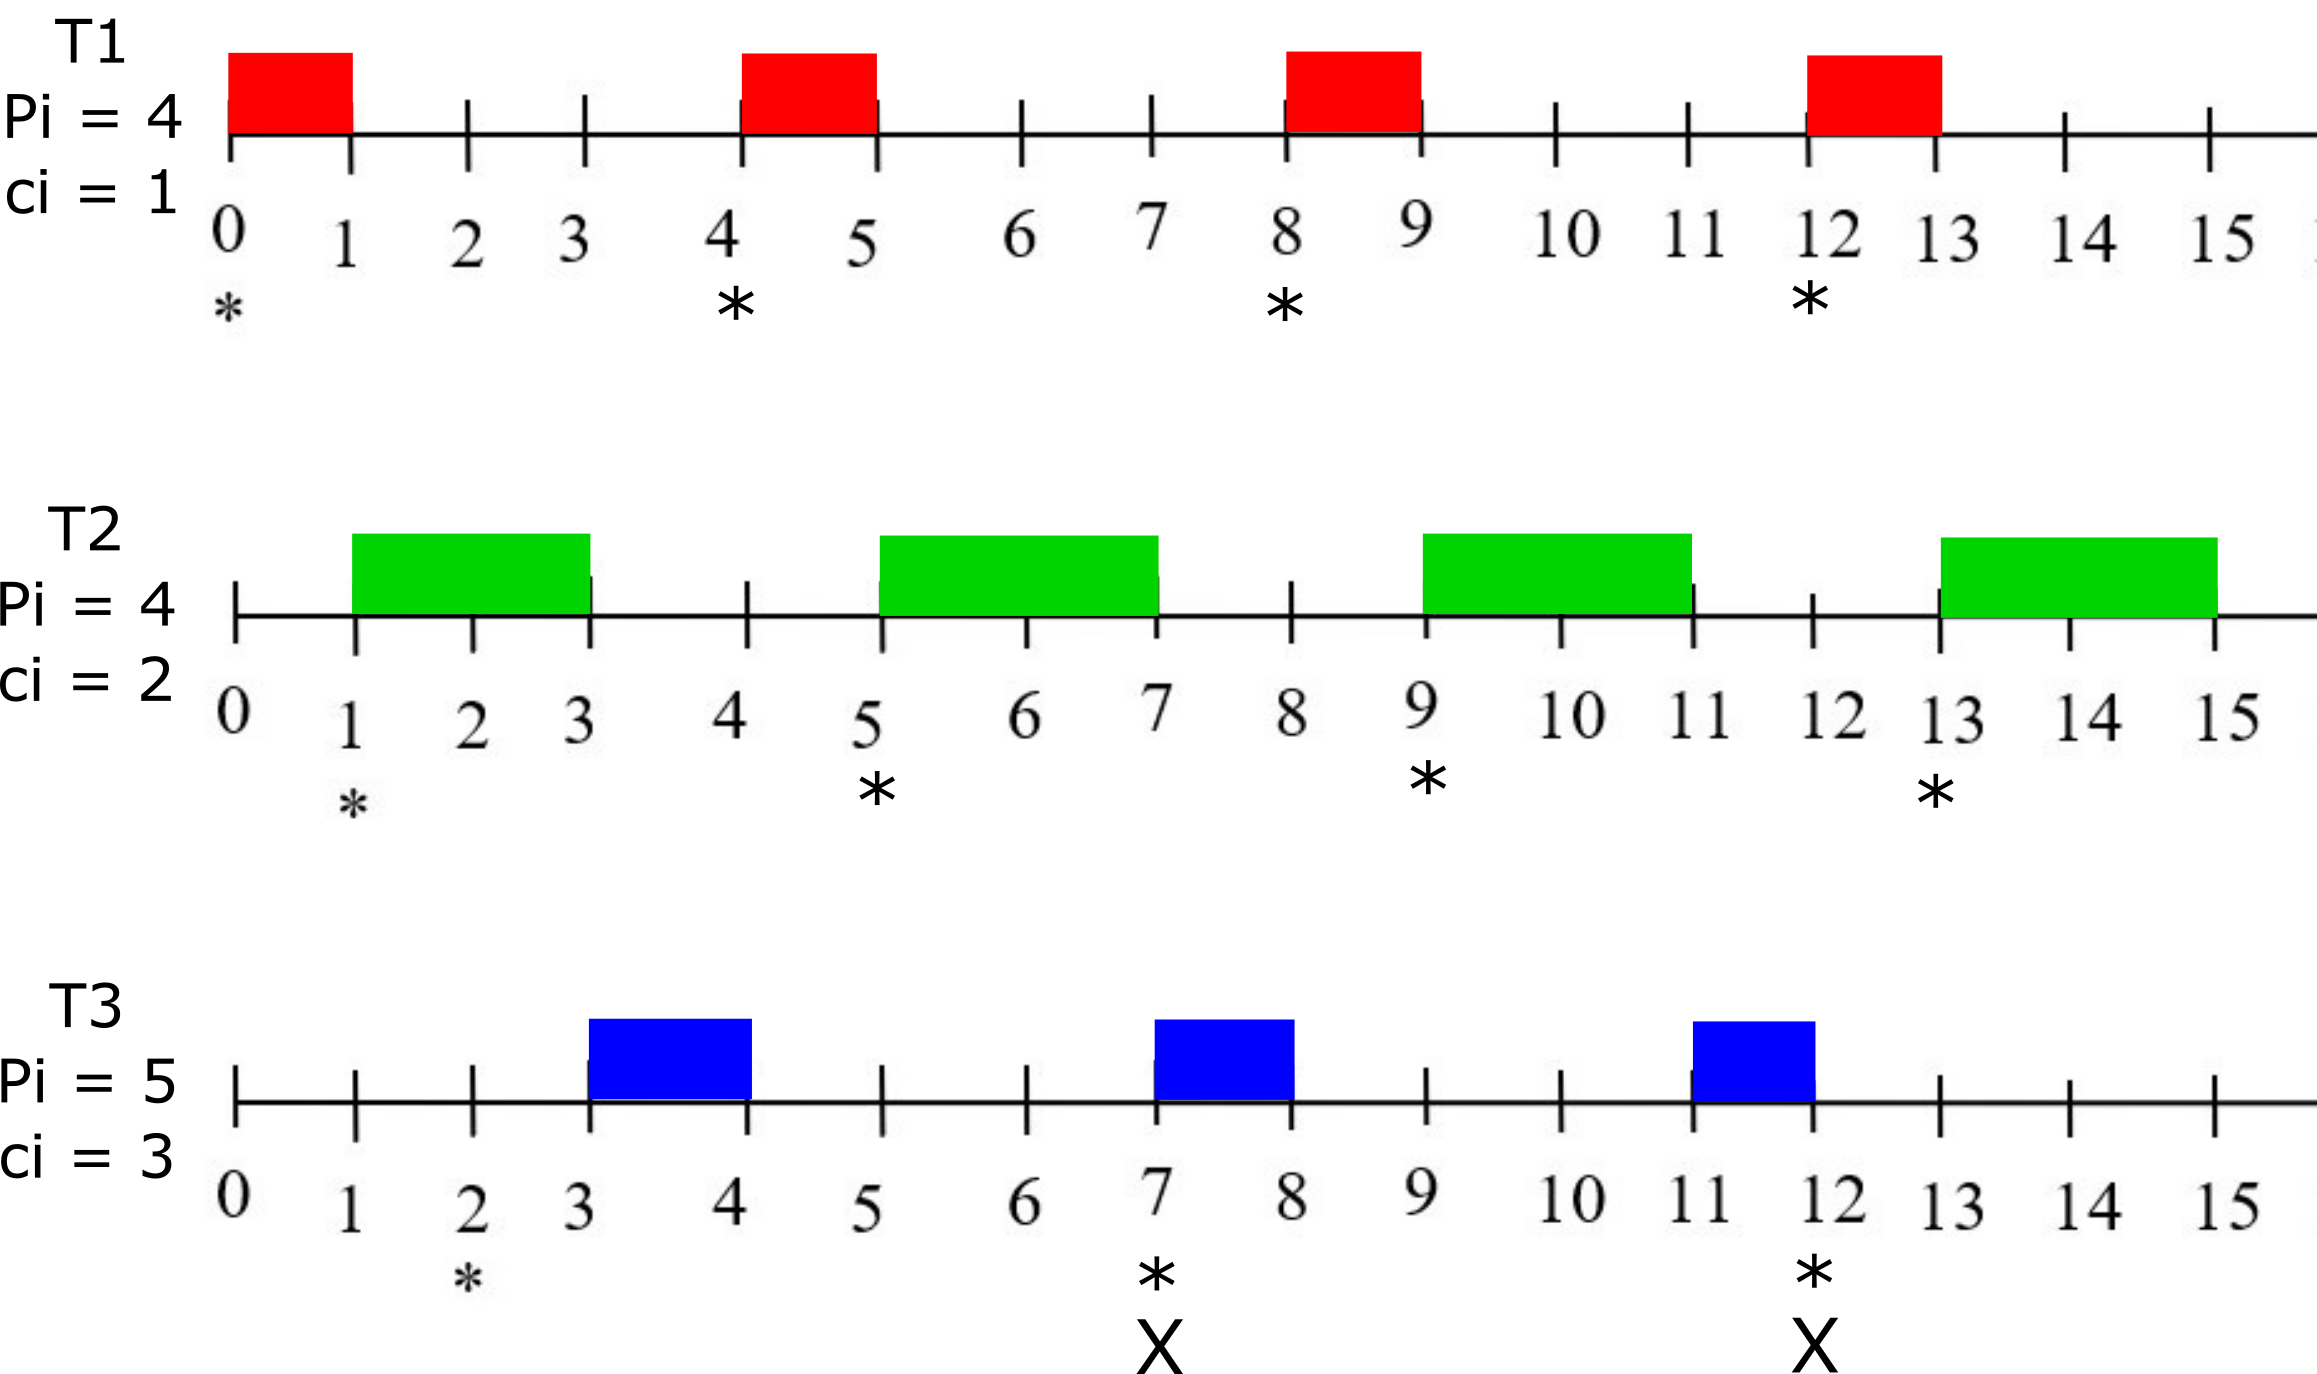
\includegraphics[width=0.9\columnwidth]{images/rmsed.png}
		}
	\end{figure}
	
	%%%%%%%%%%%%%%%%%%%%%%%%%%%%%%%%%
	%%%%%%%%%%%%%%%%%%%%%%%%%%%%%%%%%    
	\newpage
	\section*{Problem 3: EDF Scheduling (4 Points)}
	
	Schedule the tasks using EDF scheduling up to 15 timesteps.
	
	
	%% TODO: add answer here
	\begin{figure}[h]
		\centering
		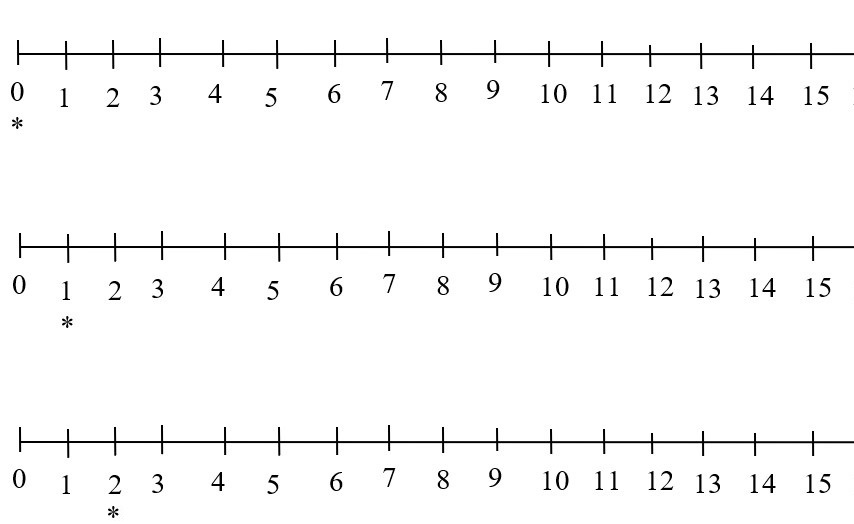
\includegraphics[width=0.8\columnwidth]{images/assignment4-timesteps.jpg}
	\end{figure}
	
	%%%%%%%%%%%%%%%%%%%%%%%%%%%%%%%%%
	%%%%%%%%%%%%%%%%%%%%%%%%%%%%%%%%%    
\end{document}
